\chapter{Implementación y Desarrollo}
\label{cap:implementacion}

Todos los detalles del código completo del proyecto pueden consultarse en el repositorio~\footnote{Repositorio de código de ClimbIt: (\url{https://github.com/Melendo/Climbit})} donde se ha llevado a cabo todo el desarrollo. Este capítulo documenta el paso de la aplicación del diseño conceptual a una solución práctica y real. Lejos de ser una descripción del código, las siguientes páginas desvelan las implementaciones tecnológicas y flujos de \textit{ClimbIt}: desde el aislamiento y la testabilidad que aporta la arquitectura hexagonal en el backend, hasta la ligereza de un frontend modular enfocado en la experiencia móvil. Asimismo, se detallará la resolución de los mayores desafíos de que han surgido durante el desarrollo del proyecto: la adaptación de la interfaz para responder correctamente en dispositivos móviles, la manipulación dinámica de mapas interactivos SVG y el diseño de una estrategia de cacheo híbrida para garantizar el funcionamiento de la app en entornos sin conectividad.

\section{Implementación del backend}

Para cumplir con los requisitos que se marcaron para el proyecto, el backend se desarrolló como una API REST 
que encapsule la lógica de negocio necesaria para gestionar los recursos principales de la aplicación y servirlos al frontend.

La implementación se organiza de forma que las responsabilidades estén claramente separadas gracias a la decisión 
de seguir una arquitectura hexagonal detallada en el capítulo de diseño. 

El alcance tratado en esta sección se limita a la implementación funcional y estructural del backend.

\subsection{Arquitectura hexagonal}

La implementación del backend sigue un enfoque de arquitectura hexagonal, representado en la figura \ref{fig:arquitectura-hexagonal}, que favorece la separación de responsabilidades, 
facilita el testing y mejora la mantenibilidad del código. Cada capa tiene un rol específico y bien delimitado:

    \begin{figure}[h]
    \centering
    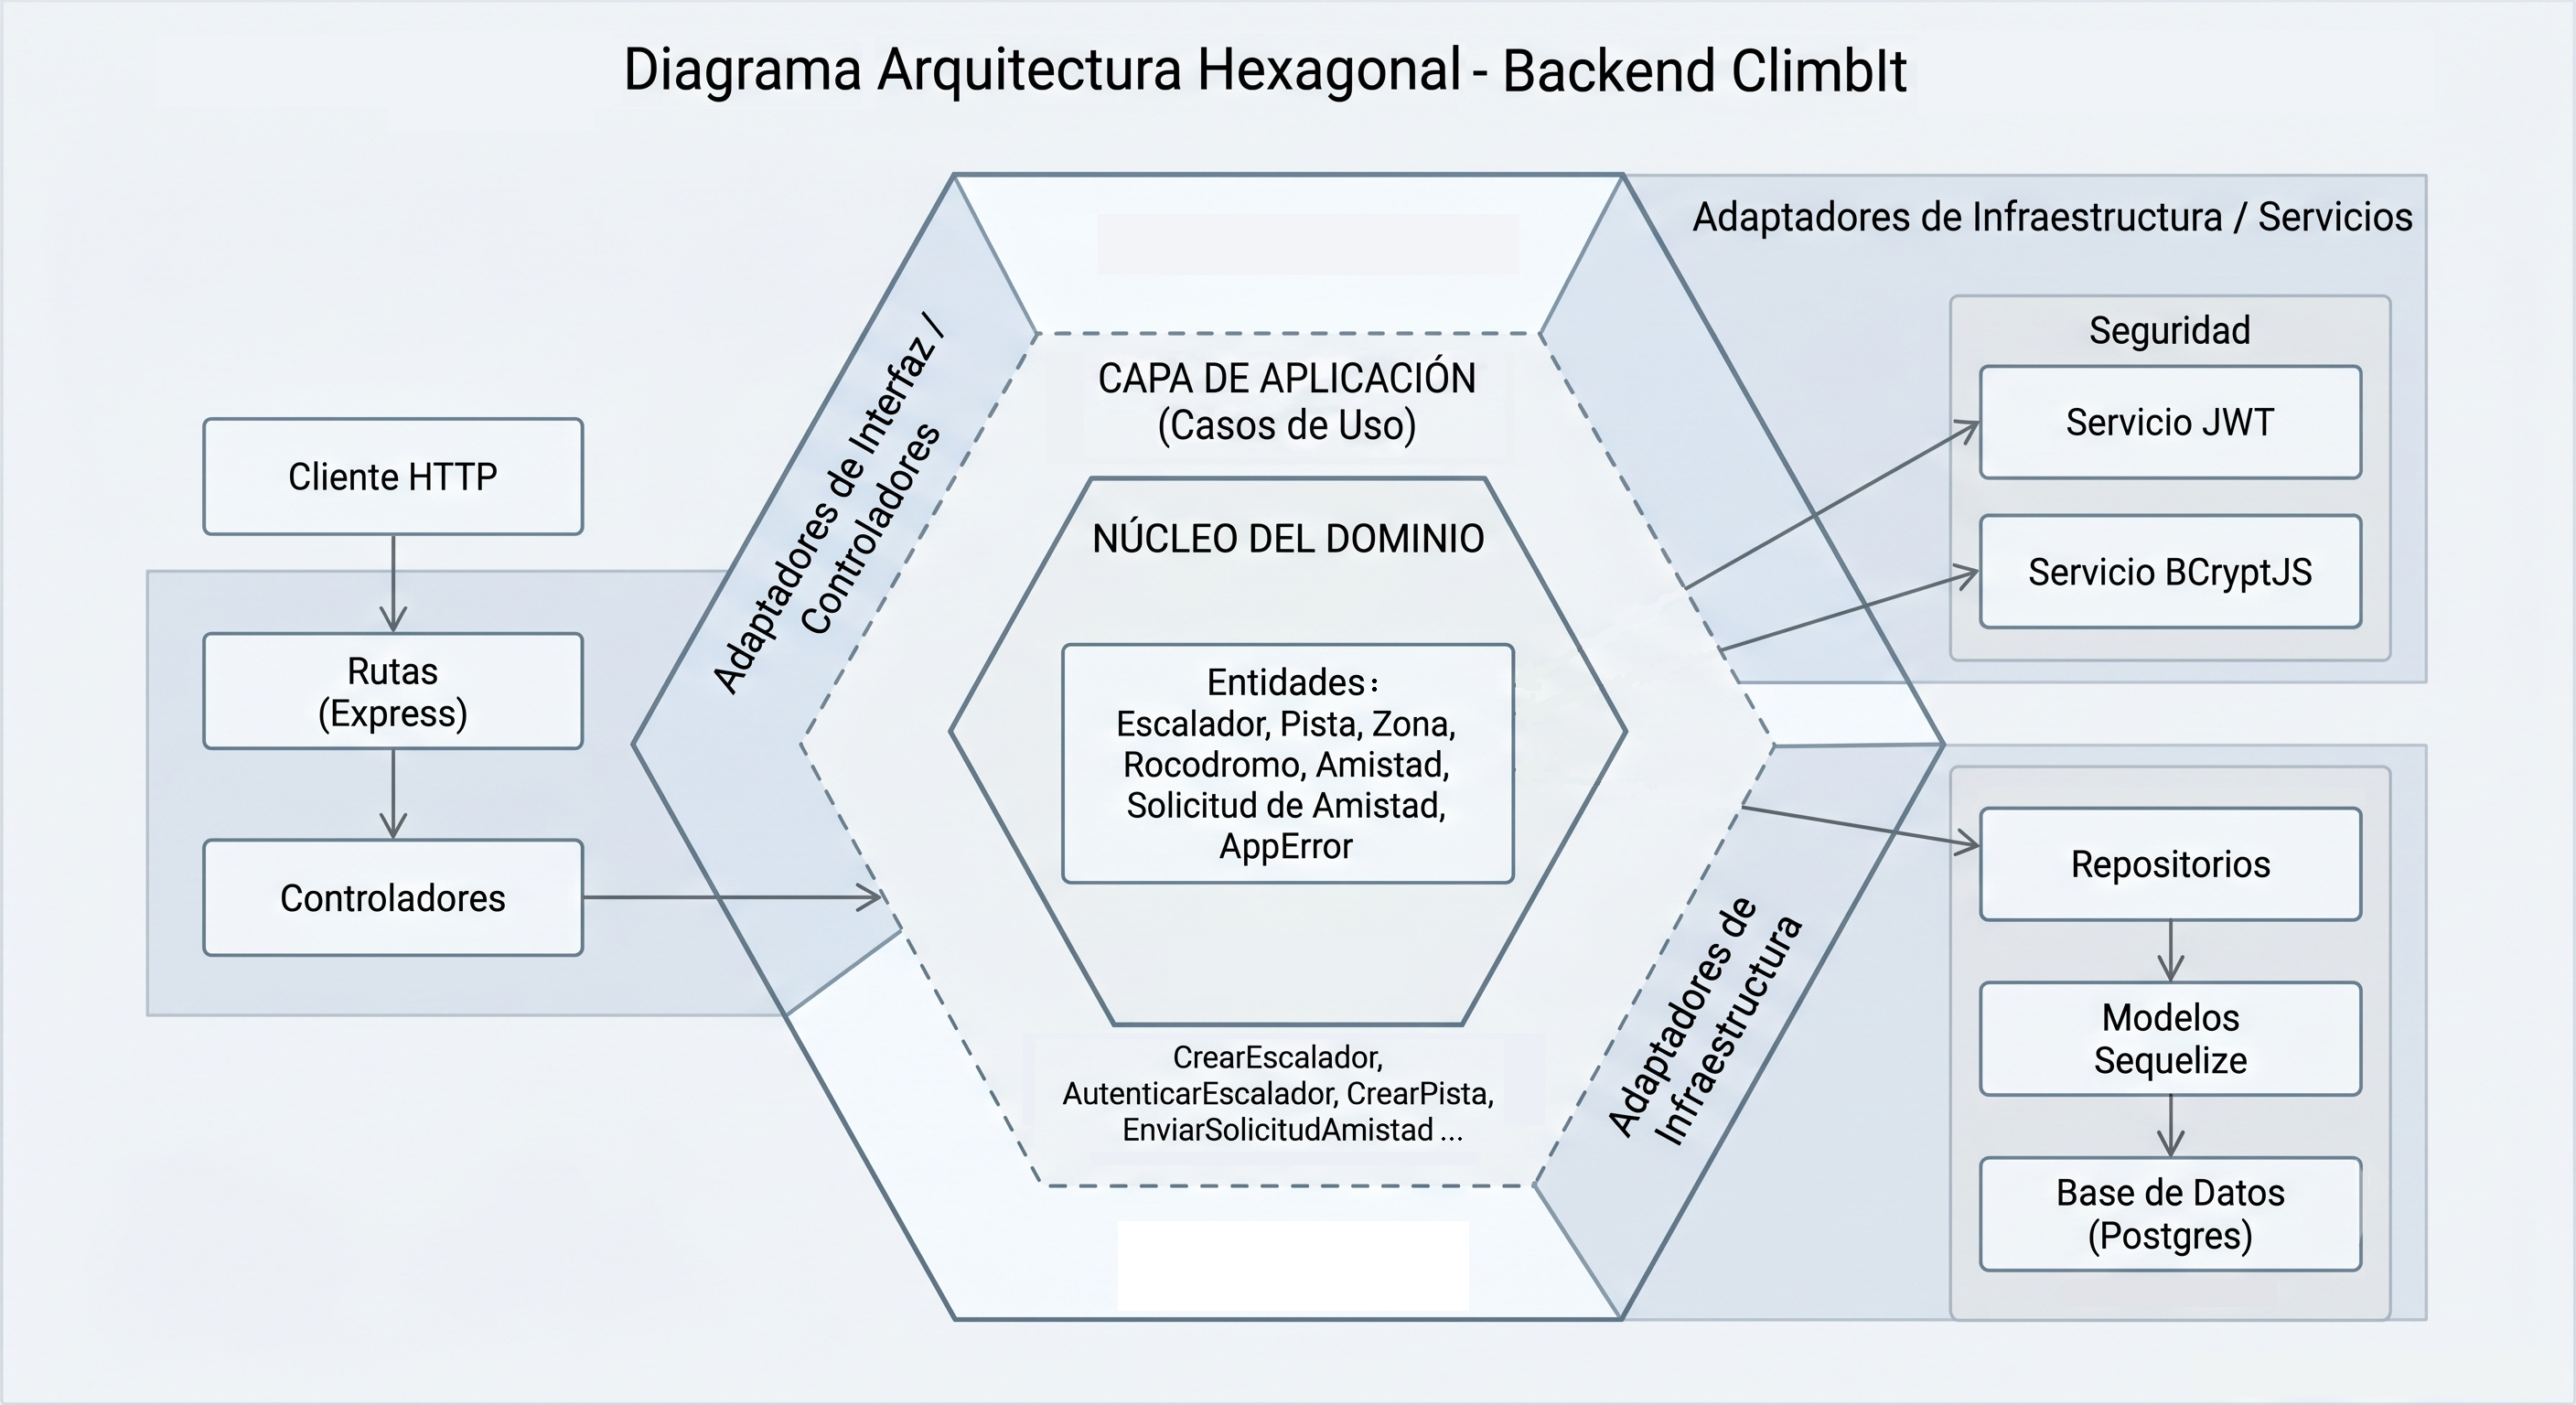
\includegraphics[width=1\textwidth]{./Imagenes/Fuentes/arquitectura_hexagonal.png}
    \caption{Arquitectura hexagonal del backend.}
    \label{fig:arquitectura-hexagonal}
    \end{figure}

\subsubsection{\textit{Domain} — Entidades y Contratos}

La capa de dominio contiene las definiciones de las entidades de negocio y las interfaces de los repositorios. 
Esta capa es independiente de cualquier tecnología específica y sin dependencias externas. Define qué es un y como se
valida un escalador, un rocódromo, etc., así como las operaciones que se pueden realizar sobre ellas a través de 
las interfaces de repositorio. 

Por ejemplo, el repositorio de escaladores define un contrato que especifica que debe existir un método 
\textit{encontrarPorCorreo(correo)} para buscar un escalador por correo, o \textit{encontrarPorApodo(apodo)} para búsquedas 
por apodo. La implementación concreta de estos métodos la proporciona la capa de infraestructura, pero el contrato se define
en esta capa.

\subsubsection{\textit{Application} — Casos de Uso}

Los casos de uso encapsulan toda la lógica de negocio de la aplicación. Cada caso de uso representa una acción que el usuario 
puede realizar como crear un escalador, autenticarse, suscribirse a un rocódromo, enviar una solicitud de amistad... Los 
casos de uso reciben repositorios y servicios a través de inyección de dependencias, realizan validaciones y orquestación, 
y devuelven resultados o lanzan excepciones, que se devuelven al controlador, que será el encargado de manejar la respuesta.

Por ejemplo, el caso de uso \textit{src/aplication/escaladores/crearEscalador.js}
recibe el repositorio de escaladores y el servicio de hash de contraseñas. El caso de uso se encarga de validar que el 
correo sea único realizando una consulta a la bd a través del repositorio, genera un hash de la contraseña usando el servicio
\textit{/infrastructure/security/passwordService.js},
crea una entidad escalador y delega la persistencia al repositorio invocando el método correspondiente, en este caso
\textit{escaladorRepository.crear(nuevoEscalador)}. Si algo falla, lanza una 
excepción descriptiva que el controlador captura y transforma en una respuesta HTTP adecuada.

\subsubsection{\textit{Infrastructure} — Implementaciones Concretas}

La capa de infraestructura contiene las implementaciones concretas de los repositorios, también llamados adaptadores. Estos son
los encargados de actuar sobre la base de datos usando Sequelize. En esta capa también se ubican servicios de utilidad, como
hashing de contraseñas mediante bcryptjs y la generación de JWT a través de jsonwebtoken, y el contenedor de inyección de 
dependencias (\texttt{container.js}). 

Aquí es donde se instancian los objetos, se conectan entre sí (un caso de uso recibe un repositorio y un servicio inyectados) 
y se exportan para su uso en las rutas. Esta capa es la que más cambiaría en caso de necesitar una arquitectura diferente: 
p. ej. cambiar de Sequelize a TypeORM, o de Postgres a MongoDB. Los casos de uso no cambiarían, solo sus dependencias 
inyectadas.

Un ejemplo: \texttt{EscaladorRepositoryPostgres} implementa la interfaz del dominio y usa Sequelize para ejecutar queries 
para persistir los datos en la bd o leerlos. 
Cuando el caso de uso llama a \textit{encontrarPorCorreo(correo)}, este repositorio traduce la operación a una consulta 
Sequelize, que a su vez la traduce a una sentencia SQL y devuelve el escalador encontrado o \textit{null} si no existe.

\subsubsection{\textit{Interfaces} — Adaptadores HTTP}

La capa de interfaz expone la aplicación mediante endpoints HTTP y está compuesta por rutas y controladores. En esta capa,
el router valida la petición, mientras que el controlador invoca el caso de uso y traduce su resultado
a una respuesta HTTP.

El flujo general de una petición es:

\begin{enumerate}
  \item El router recibe la petición HTTP con los parámetros (body, query, params).
  \item Valida los parámetros con \texttt{express-validator} y el resto de middlewares de la ruta.
  \item Redirige al controlador.
  \item Invoca el caso de uso correspondiente con los datos validados.
  \item Maneja excepciones del caso de uso y las traduce a códigos HTTP.
  \item Retorna el resultado serializado a JSON.
\end{enumerate}

Por ejemplo, el router \textit{escaladorRouter.js} procesa las llamadas a \textit{POST /escaladores/create}. Esta petición 
contiene el payload con los datos del nuevo escalador. Tras la validación con \textit{express-validator}, la petición se
deriva al controlador \textit{EscaladorController}, que ejecuta \texttt{crearEscaladorUseCase.execute(datos)}. El caso de
uso aplica la lógica de negocio, crea el escalador y genera el token JWT de autenticación. Finalmente, el controlador
retorna \textit{201 Created} con el token, o un código de error 4xx/5xx si falla el proceso.

\paragraph{\textbf{Flujo de la petición HTTP Crear Escalador:}}

\texttt{POST /escaladores/create} payload:
\verb|{correo:"user@ci.com", apodo:"John", contrasena:"Password123"}|

\begin{enumerate}
  \item El cliente HTTP envía la petición.
  \item El servidor recibe la petición en la capa de \textit{interfaces}: el router valida los parámetros con las validaciones  definidas en el validador de la ruta. Si la Validación falla se retorna un error 400 con detalles del error (la contraseña debe incluir al menos 1 número, etc.). Si la validación es exitosa, se redirecciona al controlador.
  \item El controlador invoca el caso de uso correspondiente para crear el escalador: \texttt{CrearEscaladorUseCase.execute(\{correo, apodo, contraseña\})}.
  \item El caso de uso (capa \textit{application}) ejecuta la lógica de negocio: verifica que el correo sea único consultando el repositorio; si existe, lanza excepción. Se valida que el apodo también sea único. En caso de no serlo,  lanza una excepción. Si no existe, un usuario registrado con ese apodo y ese correo, genera hash de contraseña usando el servicio y crea una entidad escalador con los datos validados.
  \item El caso de uso llama a la función concreta del repositorio para crear un nuevo escalador: \texttt{escaladorRepository.create(nuevoEscalador)}.
  \item El repositorio (capa \textit{infrastructure}) traduce a una operación Sequelize: crea un nuevo registro en la   tabla de escaladores en Postgres.
  \item Si la inserción del escalador fue exitosa, retorna al caso de uso los datos del escalador creado, y este delega de nuevo en el servicio correspondiente la generación del JWT. Si todo sale como se espera, se retorna el token al controlador.
  \item El controlador retorna un código \textit{201 Created} con el token generado o la procesa las excepciones lanzadas para retornar un error con un mensaje descriptivo.
\end{enumerate}

\subsection{Composición e inyección de dependencias}

El contenedor de inyección de dependencias se encuentra implementado en el archivo \textit{src/infrastructure/container.js} y es el punto central donde se instancian todos los objetos de la aplicación y se les inyectan las dependencias necesarias. Este patrón permite que los repositorios, casos de uso y controladores no tengan que crear directamente sus dependencias, sino que las reciben ya construidas como se comentó en capitulo \ref{cap:disenoSistema} sección de decisiones de diseño.

\paragraph{\textbf{Estructura del contenedor:}}

El contenedor es una función asíncrona que:

\begin{enumerate}
  \item Espera a que se carguen los modelos de Sequelize desde la base de datos.
  \item Instancia los repositorios, inyectándoles el modelo correspondiente:\\ \texttt{new EscaladorRepositoryPostgres(db.Escalador)}.
  \item Instancia los otros servicios de infraestructura: \texttt{passwordService}, \texttt{tokenService}.
  \item Instancia cada caso de uso, inyectándole el repository y las dependencias que utilice:\\ \texttt{new CrearEscalador(escaladorRepository, passwordService, tokenService)}..
  \item Instancia los controladores, inyectándoles los casos de uso relacionados con la entidad que representan agrupados.
  \item Exporta los controladores para ser utilizados por los routers al ercibir las peticipones HTTP correspondientes.
\end{enumerate}

\paragraph{Ventajas de este enfoque:}

\begin{itemize}
  \item \textbf{Testabilidad}: en tests unitarios, se puede pasar un mock del repositorio al caso de uso, sin tocar la base de datos real.
  \item \textbf{Flexibilidad}:  en caso de ser necesario cambiar la implementación del repositorio a, por ejemplo, otro SGBDR, únicamente 
  se requiere cambios en el contenedor y en la clase la implementación concreta del repositorio, no en los casos de uso.
  \item \textbf{Centralización}: todas las dependencias e instancias se crean en un único lugar, facilitando el mantenimiento y la visualización de dependencias.
\end{itemize}

\subsection{Manejo de errores}

La gestión de errores en ClimbIt implementa una jerarquía personalizada de excepciones que permite traducir sin fricción los errores técnicos de capas inferiores, como pueden ser errores de base de datos o validación, a errores de dominio que finalmente se transforman a respuestas HTTP coherentes.

\subsubsection*{Jerarquía de errores personalizados}

Se define una clase base \texttt{AppError} que extiende de la clase \texttt{Error} nativa de JavaScript. Esta clase encapsula:

\begin{itemize}
  \item \textbf{statusCode}: código HTTP a retornar (400, 401, 403, 404, 409, 500).
  \item \textbf{code}: identificador de error semántico (p. ej. \texttt{NOT\_FOUND}, \texttt{CONFLICT}, \texttt{VALIDATION\_ERROR}).
  \item \textbf{message}: descripción legible para el cliente.
  \item \textbf{isOperational}: indica si es un error esperado (true) o un bug del sistema (false).
  \item \textbf{cause}: referencia al error original para debugging (útil en desarrollo).
\end{itemize}

A partir de \texttt{AppError}, se definen subclases específicas:

\begin{itemize}
  \item \textbf{BadRequestError}: 400. Parámetros de entrada inválidos.
  \item \textbf{ValidationError}: 422. Validación de datos fallida.
  \item \textbf{AuthenticationError}: 401. Token JWT inválido o expirado.
  \item \textbf{AuthorizationError}: 403. Rol o permisos insuficientes.
  \item \textbf{NotFoundError}: 404. Recurso no existe.
  \item \textbf{ConflictError}: 409. Violación de regla de negocio (correo duplicado, etc.).
  \item \textbf{InternalServerError}: 500. Error inesperado (isOperational=false).
\end{itemize}

\subsubsection*{Patrón Adapter: Traducción de errores de repositorio}

Sequelize puede lanzar excepciones específicas como \texttt{SequelizeUniqueConstraintError} o \texttt{SequelizeValidationError}, cuyo contenido no es de utilidad a los casos de uso o al cliente, por lo que se traducen mediante un adaptador: la función \texttt{mapRepositoryError()} localizada en \texttt{infrastructure/repositories/dbErrorHandler.js}. Esta función:

\begin{enumerate}
  \item Recibe el error original lanzado por Sequelize.
  \item Detecta el tipo de error inspeccionando su nombre y mensaje.
  \item Traduce a la clase \texttt{AppError} correspondiente:
    \begin{itemize}
      \item Sequelize UNIQUE CONSTRAINT → \texttt{ConflictError} (409).
      \item Sequelize VALIDATION ERROR → \texttt{ValidationError} (422).
      \item Otros errores BD → \texttt{InternalServerError} (500).
    \end{itemize}
  \item Preserva el error original en la propiedad \texttt{cause} para trazabilidad en caso de ser necesario.
  \item Retorna la excepción de dominio mapeada.
\end{enumerate}

\subsubsection*{Middleware de manejo de errores HTTP}

En el archivo \texttt{src/interfaces/http/server.js} se han definido dos middlewares de captura de errores 
que se ejecutan secuencialmente:

\textbf{Errores de Multer y de Carga de archivos}

Intercepta errores específicos del procesamiento de archivos:

\begin{itemize}
  \item \texttt{MulterError} con code \texttt{LIMIT\_FILE\_SIZE}: archivo excede tamaño máximo (413 Payload Too Large).
  \item Errores de validación de tipo MIME o FFmpeg: retorna 400 Bad Request o el status definido en el error.
\end{itemize}

\textbf{Manejo genérico de AppError}

Es el punto de salida final donde todos los errores capturados en la aplicación se traducen a respuestas JSON:

\begin{enumerate}
  \item Detecta si el error es instancia de \texttt{AppError}.
  \item Si es AppError: extrae su \texttt{statusCode} y \texttt{code}.
  \item Si no: asume 500 Internal Server Error.
  \item Construye la respuesta JSON y la devuelve con el statusCode correspondiente.
\end{enumerate}


\subsubsection*{Ventajas de este enfoque de manejo de errores:}

\begin{itemize}
  \item \textbf{Separación de concerns}: Los errores no contaminan lógica de negocio.
  \item \textbf{Consistencia}: Todas las respuestas de error siguen el mismo formato JSON.
  \item \textbf{Testabilidad}: Se puede mockear errores específicos para utilizarlos en tests.
  \item \textbf{Debugging}: Se preserva el error original en \texttt{cause} sin exponerlo al cliente.
  \item \textbf{Escalabilidad}: Añadir nuevos tipos de error es trivial: extender AppError y mapear en dbErrorHandler.
\end{itemize}

\subsection{Autenticación y seguridad}

\textbf{Flujo de autenticación:}

La autenticación en la aplicación se implementa mediante JWT (JSON Web Tokens). El flujo es:

\begin{enumerate}
  \item El usuario intenta iniciar sesión proporcionando correo, contraseña.
  \item El caso de uso \texttt{AutenticarEscalador} recupera el escalador por correo.
  \item Compara la contraseña proporcionada con el hash almacenado en la base de datos usando \texttt{bcryptjs.compare()}.
  \item Si coincide, genera un JWT firmado con una clave secreta, incluyendo correo, el apodo y el rol: Escalador, Admin o Gestor. En caso de ser gestor, se incluye un array con los ids de los rocódromos que gestione.
  \item El cliente almacena el JWT para enviarlo en el header \texttt{Authorization: Bearer <token>} de futuras peticiones.
\end{enumerate}

\paragraph{Middleware de autenticación:}

Cada ruta protegida (p. ej. obtener perfil, actualizar datos) valida que exista un JWT válido antes de procesar la petición. Si el token es inválido o expirado, se retorna 401 Unauthorized. Todas las rutas salvo las de inicio de sesión y registro se encuentran protegidas y deben pasar esta validación para continuar.

\textbf{Validaciones de entrada:}

Todas las rutas validan los parámetros de entrada usando \texttt{express-validator}. Algunas de las validaciones que se realizan son las siguientes:

\begin{itemize}
  \item \textbf{Correos}: validación de formato de email.
  \item \textbf{Contraseñas}: longitud mínima, tipos de caracteres...
  \item \textbf{IDs}: validación de que sean números o UUIDs según el formato esperado.
  \item \textbf{Archivos}: validación de MIME-type y tamaño máximo.
\end{itemize}

Las validaciones fallidas retornan un código 422 Invalid Request con detalles de error que lo produce(p.e. longitud de la contraseña insuficiente) o 500 Internal Server Error si en el proceso de subir una imagen se suceden errores.

\paragraph{Consideraciones de seguridad:}

\begin{itemize}
  \item Las contraseñas nunca se almacenan en texto plano.
  \item Los tokens JWT tienen un tiempo de expiración de 12h para mitigar riesgos de compromiso.
  \item Los secretos (clave de JWT, credenciales de la bd) se almacenan en variables de entorno, nunca en el código.
  \item Los errores de autenticación no revelan si el correo existe o no, para prevenir enumeración de usuarios.
\end{itemize}

\subsection{Gestión de archivos multimedia}

A través del middleware \texttt{Multer} se reciben los archivos de tipo \texttt{multipart/form-data} en el backend. Una vez obtenidos se les pasa una primera validación de MIME-type y tamaño máximo de los archivos como filtro antes de proceder a una evaluación más exhaustiva. Una vez superada esa primera validación, a través de la librería \texttt{file-type} se obtiene el tipo real del archivo leyendo sus \textit{magic bytes} para prevenir posibles brechas de seguridad con los archivos recibidos. 

Una vez validadas se convierten al formato WebP utilizando \texttt{FFmpeg}, garantizando una comprensión eficiente que permite reducir su tamaño sin perdida de calidad apreciable. Esto se traduce en una mejora de rendimiento a la hora de servir las imágenes y un menor consumo de espacio en disco.

Si el endpoint al que se intenta subir una imagen es \texttt{POST /zonas/:id/mapa}, el flujo cambia. Se valida que el formato sea svg exclusivamente. Cualquier otro formato es rechazado por decisión técnica de negocio. Estos mapas se renderizan en el frontend y se requiere que sean vectoriales para mantener su calidad al manipularlos desde la interfaz. Por ende, estas imágenes tampoco son procesadas por FFmpeg, sino que se almacenan directamente en formato svg después de validar su tipo real con \texttt{file-type}.


\paragraph{Tipos de archivos gestionados:}

La aplicación  y sirve dos tipos de archivos, svg para los mapas de las zonas y webp para el resto de imágenes. Todas
las imágenes se almacenan en distintas carpetas dentro del directorio \texttt{/app/backend/uploads/} según la entidad a la que
pertenecen:

\begin{itemize}
  \item \textbf{Fotos de perfil}: \texttt{/uploads/fotos\_perfil/}.
  \item \textbf{Imágenes de rutas}: \texttt{/uploads/imagenes\_pistas/}.
  \item \textbf{Logos de rocódromos}: \texttt{/uploads/logos\_rocodromos/}.
  \item \textbf{Mapas de zonas}: \texttt{/uploads/mapas\_zonas/}.
\end{itemize}

\paragraph{Seguridad en archivos:}

\begin{itemize}
  \item \textbf{Validación de tipo}: Se usa la librería \texttt{file-type} para verificar la firma real del archivo y no confiar solo en el MIME ni en la extensión.
  \item \textbf{Límite de tamaño}: Previene ataques de denegación de servicio (llenado de disco).
  \item \textbf{Nombres sanitizados}: Los archivos se renombran para evitar problemas de seguridad y privacidad.
  \item \textbf{Almacenamiento seguro}: Los archivos se sirven a través de rutas controladas, no directamente del filesystem.
\end{itemize}

\subsection{Testing y calidad}

La calidad es uno de los pilares clave que se marcaron para el desarrollo del proyecto. Al trabajar con unos 
requisitos cambiantes en las iteraciones se quería garantizar la robustez de la aplicación. Por ello, se implementó 
una estrategia de pruebas en dos niveles: tests unitarios, para probar la lógica de las diferentes capas de forma aislada,
y test E2E (\textit{end-to-end}) para validar los flujos completos de las peticiones HTTP.

\begin{itemize}
  
\item Los \textbf{tests unitarios} validan los casos de uso de forma aislada, usando mocks de los repositorios y de los casos de uso 
para comprobar lógica de negocio, validaciones, manejo de errores y persistencia sin necesidad de una base de datos real.


\item Los \textbf{tests e2e} cubren flujos completos de las funciones reales de la aplicación. 
Se cubren todos los casos posibles especificados en las Historias de Usuario. Los tests E2E se ejecutan contra bases de datos
idénticas a las de producción gracias a las migraciones de Sequelize. 
\end{itemize}

Para realizar los test se ha utilizado la librería \texttt{Jest} que permite el uso de mocks y aserciones, perfectamente 
integrable en la arquitectura implementada. En el caso de los test E2E, se ha utilizado \texttt{supertest} para simular 
peticiones HTTP a la aplicación y validar las respuestas. 

Para garantizar el nivel de calidad propuesto para el proyecto y eliminar riesgos de errores al refactorizar y añadir funcionalidades, se estableció una política de cobertura de código mínima del 80\% en líneas, ramas y funciones en todos los archivos,
excluyendo archivos de configuración, migraciones y modelos de Sequelize. Esta configuración se encuentra en el archivo \texttt{jest.config.js}
situado en \texttt{apps/backend}.

\subsection{Resumen}

La implementación del backend se estructura siguiendo principios de arquitectura hexagonal, garantizando 
separación de responsabilidades, testabilidad y flexibilidad.

\paragraph{Puntos fuertes de la implementación:}

\begin{itemize}
  \item \textbf{Arquitectura por capas}: Domain → Application → Infrastructure, con clara separación de concerns.
  \item \textbf{Casos de uso encapsulados}: la lógica de negocio está centralizada, facilitando cambios y reutilización.
  \item \textbf{Inyección de dependencias}: flexibilidad para cambiar implementaciones (repositorios, servicios) sin alterar casos de uso.
  \item \textbf{Seguridad}: autenticación por JWT, hashing de contraseñas con bcryptjs, análisis de imágenes con file-type 
  y validación de acceso a endpoints exhaustiva.
  \item \textbf{Mejora de rendimiento}: conversión de imágenes a WebP mediante FFmpeg para reducir los tiempos de carga 
  y el consumo de espacio.
  \item \textbf{Manejo de errores}: excepciones específicas del negocio traducidas a respuestas HTTP claras.
  \item \textbf{Testing}: estrategia multicapa con tests unitarios y e2e, umbrales de cobertura del 80\%.
  \item \textbf{Escalabilidad}: la estructura de carpetas y composición permite añadir nuevos casos de uso, repositorios y 
  controladores sin una refactorización mayor.
\end{itemize}


Esta implementación proporciona una base sólida, mantenible y escalable para el futuro de ClimbIt.


\section{Implementación del Frontend}

La implementación del frontend de ClimbIt se ha enfocado en construir una interfaz web de tipo SPA (\textit{Single Page Application}) centrada en la experiencia móvil, como se trató en el capítulo anterior, con navegación basada en hash, reutilización de componentes y una integración directa con la API REST del backend para la subida de los datos de los escaladores y descarga de la información necesaria para construir las vistas. El objetivo principal ha sido ofrecer una interfaz ligera, modular y coherente, manteniendo una estructura de código fácil de mantener y de ampliar.

A diferencia del backend, donde la organización responde a una arquitectura hexagonal, en el frontend se ha planteado a una adaptación del patrón \textbf{MVC} (Modelo-Vista-Controlador) separada en 3 capas: un núcleo común de infraestructura de interfaz, módulos funcionales por dominio y una capa de componentes reutilizables. Esta división permite que cada pantalla tenga su propio controlador y su propia vista, pero comparta la lógica transversal de navegación, autenticación, peticiones HTTP y retroalimentación visual.

\subsection{Tecnologías y base de la aplicación}

El frontend se implementó con \textit{Vite} como entorno de desarrollo y construcción, \textit{Bootstrap} como base de componentes visuales y un conjunto reducido de utilidades propias para adaptar la interfaz a las necesidades del proyecto. La aplicación incorpora además soporte \textbf{PWA} mediante \texttt{vite-plugin-pwa}, lo que permite instalarla en dispositivos móviles y aprovechar el uso de caché para funcionar parcialmente sin conexión.

Los estilos de la aplicación se centralizan en \texttt{src/css/global.css}, donde se redefine la tipografía y se ajusta la paleta de colores para mantener una conisistencia visual a lo largo del proyecto. También se introducen variables CSS propias para controlar la altura útil del \textit{viewport}, el ancho máximo de la aplicación y los márgenes en distintas resoluciones de dispositivos móviles.

\subsection{Estructura general del frontend}

La carpeta \texttt{src/js} concentra toda la lógica de la aplicación y se organiza en tres bloques principales:

\begin{itemize}
  \item \textbf{core}: contiene la infraestructura transversal de la interfaz, como el router, el cliente HTTP y utilidades de UI.
  \item \textbf{modules}: agrupa la funcionalidad por dominio, con duplas controlador-vista para cada área funcional.
  \item \textbf{components}: reúne las diferentes piezas reutilizables que componen la interfaz, como modales, la barra de navegación, tarjetas, mapas SVG o \textit{helpers} de formularios.
\end{itemize}

Esta estructura evita que cada pantalla replique lógica común y permite que las vistas se construyan a partir de piezas pequeñas, focalizadas en una única responsabilidad.

\subsection{Punto de entrada, navegación y ciclo de vida}

El archivo \texttt{src/js/app.js} actúa como punto de entrada de la aplicación. En él se registran los \textit{service workers} de la PWA, se inicializa el router, se activa el banner de conectividad y se ajusta dinámicamente la variable \texttt{--vh} para corregir problemas de altura en distintos navegadores móviles. Además, cuando la aplicación se ejecuta instalada como PWA, se intenta bloquear la orientación en modo vertical para reforzar la experiencia de uso pensada para teléfonos.

El enrutado es implementado en \texttt{src/js/core/router.js} mediante \textit{hash routing}. Cada pantalla se identifica por un fragmento de URL como \texttt{\#login}, \texttt{\#perfil}, \texttt{\#misRocodromos} o \texttt{\#mapaZona?id=1\&zona=2}. El router interpreta la ruta después del \texttt{\#}, extrae los parámetros de la url, si los posee, y aplica restricciones de acceso según el estado de autenticación y los permisos del usuario. Las rutas públicas se limitan a inicio, login y registro, mientras que el resto de pantallas de la aplicación se encuentran limitadas y requieren un token válido.

De esta manera el flujo de navegación queda centralizado en un único punto: el router decide qué controlador tiene que ejecutar, el controlador recupera datos y aplica la lógica necesaria para llevar a cabo la acción correspondiente, y la vista genera el HTML final a través de fragmentos de código propios y componentes reutilizables. Este patrón simplifica la trazabilidad del comportamiento y reduce la dependencia entre pantallas.

\subsection{Cliente HTTP y gestión de autenticación}

La comunicación con el backend se abstrae a un único punto encapsulado en \texttt{src/js/core/client.js}, donde se encapsula la función \texttt{fetchClient()}. Este cliente añade el token JWT al encabezado \texttt{Authorization}, gestiona el modo sin conexión y unifica el tratamiento de errores de red y de respuesta HTTP.

Cuando el servidor responde con un código \textit{401 Unauthorized}, el cliente interpreta que la sesión ha caducado o que el token es inválido, por lo que procede a eliminar las credenciales almacenadas y redirigir de nuevo al login. De esta forma, la lógica de sesión queda centralizada y no es necesaria replicarla en cada módulo.

Además, desde el frontend se distingue entre peticiones de solo lectura (\texttt{GET, HEAD, OPTIONS}) y peticiones de escritura (\texttt{POST, PUT, PATCH, DELETE}). Si el dispositivo está offline, las operaciones modificadoras se bloquean, mientras que las peticiones de lectura pueden seguir dependiendo del estado de la aplicación y de la información almacenada en caché de la PWA. Esta decisión refuerza el modo lectura sin conexión y evita que el usuario intente ejecutar cambios que el backend no podría persistir.

La autenticación se apoya en las funciones \texttt{saveToken()}, \texttt{removeToken()} y \texttt{getTokenPayload()}, que permiten almacenar el JWT, destruirlo, recuperarlo y decodificar su contenido para aplicar reglas de acceso por rol. Esto se utiliza, por ejemplo, para verificar si un usuario puede gestionar un rocódromo antes de habilitar ciertas acciones en la interfaz.

\subsection{Organización por módulos funcionales}

Cada dominio de la aplicación es un módulo independiente con dos piezas principales: el controlador y la vista. Los controladores contienen la lógica de interacción, realizan las peticiones al backend y preparan los datos; las vistas reciben esos datos y generan el HTML correspondiente para formar la interfaz.

La aplicación se divide en los siguientes módulos:

\begin{itemize}
  \item \textbf{autenticacion}: login y registro en varios pasos.
  \item \textbf{home}: pantalla de entrada y redirección según el estado de sesión. Actualmente es la vista de Mis Rocódromos.
  \item \textbf{escalador}: información de perfil, edición de datos y estadísticas personales de desempeño.
  \item \textbf{rocodromo}: listado de rocódromos, búsqueda, detalle, suscripciones, edición y estadísticas.
  \item \textbf{zona}: mapa SVG interactivo de una zona con selección de rutas, filtros, \textit{progress bar} y listado de rutas presentes en el mapa.
  \item \textbf{ruta}: creación, modificación, detalles, estado con respecto al escalador y valoraciones.
  \item \textbf{social}: listado de amigos, solicitudes y ranking mensual con tus amistades.
  \item \textbf{error}: página de error o de recursos no encontrados.
\end{itemize}

Este modelo una evolución autónoma conforme se amplíen las funcionalidades y una separación lógica y física de responsabilidades. Por ejemplo, el flujo de registro no comparte estado con el módulo de perfil, y la lógica de mapas SVG se concentra solo en \texttt{zona} y los componentes asociados.

\subsection{Interfaz de usuario y componentes reutilizables}

Para evitar duplicar código en componentes visuales y de interacción, se definió una capa de componentes, que es compartida para todos los módulos y ubicados en \texttt{src/js/components}. Entre los elementos más relevantes se encuentran:

\begin{itemize}
  \item \textbf{navbar.js}: navegación inferior adaptada a la versión móvil de la aplicación.
  \item \textbf{modal.js} y \textbf{toast.js}: modales de confirmación de acciones (p.e. eliminar un amigo) y avisos transitorios para retroalimentación al usuario (p.e. confirmación de solicitud de amistad enviada).
  \item \textbf{svgPanzoomMap.js}: interacciones con los mapas SVG.
  \item \textbf{climbingConfig.js}: configuraciones comunes de diferentes módulos como escalas, colores y normalización de estados.
  \item \textbf{formHelpers.js}, \textbf{editableField.js} y otros helpers: componentes de apoyo para formularios e inputs aislados, como los de edición de perfil.
\end{itemize}

La existencia de estos componentes reduce la complejidad de las vistas. En lugar de implementar lógica para cada una de las vistas, se reutilizan piezas ya preparadas para renderizar tarjetas, divisores, botones de estado o indicadores de rutas, permitiendo así mantener una consistencia visual para elementos similares y un código más limpio.

\subsection{Diseño responsive, móvil y PWA}

La aplicación se ha diseñado pensando primero en móvil. El contenedor principal centra el contenido en escritorio con un ancho máximo acotado, pero en pantallas pequeñas se adapta a toda la anchura disponible y aprovecha la altura completa del dispositivo. Esta decisión encaja con el uso esperado de ClimbIt como acompañante en rocódromos a través de dispositivos móviles.

El soporte PWA añade la posibilidad de instalar la aplicación y obtener así un modo de uso más cercano a una app nativa. Junto a ello, el frontend muestra un banner de conectividad que informa cuando no hay red y pasa la aplicación a estar en modo lectura. Todo ello se complementa con la gestión de la variable \texttt{--vh}, que corrige desajustes de altura causados por la interfaz del navegador móvil.

\subsection{Estilo visual y coherencia de interfaz}

El diseño visual se controla desde \texttt{global.css}, donde se ajustan colores, tipografía y estilos específicos de la aplicación. Además de redefinir el color primario de Bootstrap, se introducen estilos para  cada componente y sección de la aplicación: \textit{cards}, barra de navegación, botones de estado de ruta, etc.

La coherencia visual se apoya en dos decisiones: por un lado, reutilizar Bootstrap como base estructural; por otro, introducir una capa de personalización propia centrada en los diseños marcados tras el análisis de los requisitos y formulados en el apartado de \textit{Diseño de la IU y UX}. Esto permite obtener una interfaz reconocible sin perder flexibilidad cuando se necesitan patrones específicos como mapas, indicadores de dificultad o estados de ruta.

\subsection{Calidad y verificación}

Para el frontend no se ha implementado una estrategia de testing automatizado, sino que se ha optado por una validación manual de las Historias de Usuario sumada a la ejecución de pruebas regresivas en las zonas afectadas por la adición de nuevas funcionalidades. Debido a la naturaleza iterativa del proyecto sujeta a las validaciones de los usuarios y la implementación progresiva de las funcionalidades, se consideró que la adopción y mantenimientos de un sistema automatizado de testing sería contraproducente debido al esfuerzo de implementación y mantenimiento requerido en contraposición al alcance establecido. La estructura de estas pruebas se basa en la ejecución de flujos concretos de las funcionalidades implementadas alineadas con los criterios de aceptación de las Historias de Usuario, desglosadas en el \textit{Apéndice A}. Si bien no se han implementado pruebas automáticas a este punto, sí se plantea en la sección de \textit{Conclusiones y trabajo futuro} como una línea de mejora una vez se estabilicen los requisitos y el proyecto alcance un nivel de madurez suficiente.

\subsection{Resumen}

La implementación del frontend de ClimbIt se apoya en una SPA modular, ligera y orientada completamente a dispositivos móvil, con un router central, un cliente HTTP común y una división clara entre módulos funcionales y componentes reutilizables.

\textbf{Puntos fuertes de la implementación:}

\begin{itemize}
  \item \textbf{Arquitectura modular}: cada dominio se encapsula en su propio módulo de controlador y vista.
  \item \textbf{Navegación centralizada}: el router controla a través del hash de la url el acceso a las pantallas.
  \item \textbf{Integración uniforme con la API}: \texttt{fetchClient()} concentra autenticación, errores y comportamiento offline de la aplicación.
  \item \textbf{Experiencia móvil}: interfaz orientada a pantallas pequeñas, navegación inferior y ajustes de viewport específicos.
  \item \textbf{Reutilización de componentes}: modales, toasts, mapas SVG y helpers reducen duplicación de código y mejoran el mantenimiento.
  \item \textbf{Coherencia visual}: estilos globales y configuración común para tipografía, paleta de colores y componentes interactivos.
  \item \textbf{Soporte PWA}: posibilidad de instalación y comportamiento mejorado en dispositivos móviles.
\end{itemize}

En conjunto, esta implementación proporciona una interfaz consistente con la lógica del backend así como el uso previsto de la aplicación por parte de los usuarios, manteniendo un equilibrio entre simplicidad técnica sin la inclusión de frameworks y riqueza funcional.

\section{Desafíos técnicos superados}

A continuación se describen los principales desafíos encontrados durante la implementación del proytecto y las soluciones que se aportaron para solventarlos.

\subsection{Adaptación de la interfaz a móvil y PWA}

Uno de los retos técnicos que se dieron a lo largo del desarrollo fue la adaptación de la interfaz para ser absolutamente responsive en distintos dispositivos móviles sin disponer de las facilidades de un framework que lo resuelve de forma nativa. Esto obligó a implementar manualmente varios comportamientos transversales a toda la aplicación para garantizar una experiencia consistente en navegadores móviles y en modo instalado como PWA. El \textit{viewport} es diferente en los navegadores debido a la barra de direcciones, el teclado virtual y la orientación del dispositivo, que produce problemas de desajustes al realizarse actualizaciones de la interfaz, por recargas o cambios de orientación.

La solución a este problema fue a través de la gestión de una variable CSS personalizada \texttt{--vh}, que se actualiza dinámicamente en eventos que afectan al \textit{viewport}, recuperándose de nuevo esa altura real y asignándola a la variable y no ver modificada la interfaz por mantener una altura fija.

\subsection{Componente de mapa SVG interactivo}

La implementación del mapa \textit{SVG} interactivo fue uno de los desafíos más exigentes del proyecto. No se trataba únicamente de mostrar una imagen, sino de construir un elemento que pudiera de responder a distintas interacciones como desplazamientos o zoom junto con actualizaciones dinámicas del contenido superpuesto en el propio mapa.

La solución implementada encapsula toda la lógica del en un componente. La gestión de eventos de interacción quedó delegada en la librería \texttt{panzoom}, que proporciona un manejo simplificado de interacciones como pan y zoom y proporciona una experiencia fluida al manipular el mapa \textit{SVG}. Para cargar el contenido de la zona correspondiente, se aprovechan los elementos cacheados previamente a la construcción del mapa, obtenidos al cargar la información para la vista, optimizando el rendimiento y evitando recargas innecesarias de los recursos. La arquitectura separa la estructura del mapa base del contenido dinámico permitiendo reutilizarlo en diferentes vistas que requieren un contenido diferente, como en la vista de creación de ruta, en la que, aparte de cargar las rutas de la zona, se añade un nuevo componente, que posiciona en un punto del mapa donde se pulse un elemento que representa la ubicación de la nueva ruta que se quiere añadir.

En resumen, la implementación del mapa \textit{SVG} requirió combinar gestión de recursos del DOM, la integración con una librería externa para la gestión de eventos de interacción y la optimización de la carga del contenido para garantizar una experiencia fluida y satisfactoria para los usuarios.


\section{Sistemas de cacheo y modo offline}

Para terminar con esta sección, uno de los retos más desafiantes fue garantizar que la aplicación siguiera siendo útil cuando el dispositivo se encuentre \textit{offline}. Para ello se definió una estrategia de cacheo híbrida que combina el almacenamiento de recursos estáticos con la persistencia local del estado de la interfaz, de forma que el usuario pueda seguir navegando por la información ya cargada aunque no pueda consultar el servidor en ese momento. Esta aproximación fue especialmente importante en una aplicación pensada para usarse en movilidad, donde la cobertura de red no siempre está asegurada.

La solución se apoyó en la capacidad de la PWA para conservar recursos previamente descargados y en la lógica común del cliente HTTP para distinguir entre operaciones de lectura y de escritura. Cuando la aplicación detecta que no hay conexión, mantiene disponibles las vistas que pueden construirse con datos ya cacheados, muestra un aviso de estado y limita las acciones que dependen de una persistencia inmediata en el backend. De este modo, el sistema conserva una parte significativa de su funcionalidad sin comprometer la coherencia de los datos.

Para evitar incoherencias entre la información local y la remota, se aplicó una política conservadora de sincronización al recuperar la conexión. En ese momento, la aplicación valida el estado de los recursos, actualiza la información necesaria y resuelve los posibles conflictos priorizando la integridad de los datos frente a la inmediatez de la actualización. Además, se controló con especial cuidado la vigencia de los elementos cacheados para equilibrar rapidez de carga y frescura de la información, evitando que el usuario trabaje con contenido obsoleto durante más tiempo del necesario.

En conjunto, este sistema de cacheo y funcionamiento offline refuerza el carácter móvil de la aplicación y aporta resiliencia frente a fallos de conectividad, manteniendo una experiencia de uso coherente incluso fuera de línea.
